\documentclass{beamer}
\usepackage{sdp}

\title{Хетерогенни контейнери}

\date{6 декември 2017 г.}

\titlegraphic{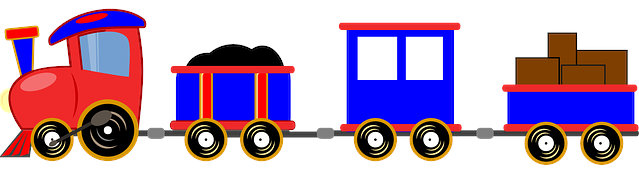
\includegraphics[height=0.35\textheight]{images/polylist.jpg}}

\begin{document}

\begin{frame}
  \titlepage
\end{frame}

\section{Дефиниция}

\begin{frame}
  \frametitle{Логическо описание}
  Контейнер, чиито елементи може да са от различен тип\\[1em]
  Операции:
  \begin{itemize}
  \item всички операции на конкретната СД (напр. стек, опашка списък)
  \item изпълняване на еднотипна операция за всеки елемент
    \begin{itemize}
    \item \textbf{Пример:} извеждане
    \item реализацията на операцията може да е различна за всеки отделен тип
    \end{itemize}
  \item изпълняване на операция само за елементи от определен тип
    \begin{itemize}
    \item \textbf{Пример:} в хетерогенен списък от хора да се повиши оценката на всички студенти
    \end{itemize}
  \end{itemize}
\end{frame}

\begin{frame}
  \frametitle{Физическо представяне}
  \newcommand{\pha}{\hspace{2ex}}
  \newcommand{\classA}{\cbox{red}{\mystrut(2.5em,2em)Клас A}}
  \newcommand{\classB}{\cbox{green}{\mystrut(1.5em,1em)Клас B}}
  \newcommand{\classC}{\cbox{yellow}{\mystrut(2em,1.5em)Клас C}}
  \begin{tabular}{*6l}
    \nextcell\pha&\nextcell\pha&\nextcell\pha&\ldots&\nextcell\pha&\nilcell\pha\\
    \bda&\bda&\bda&&\bda&\bda\\[-9pt]
    \classA&\classB&\classC&&\classB&\classA
  \end{tabular}
\end{frame}

\begin{frame}
  \frametitle{Реализация}
  Дефинира се общ базов клас (\tt{Object}) за елементите в списъка
  \begin{itemize}
  \item \tt{Object} обикновено е интерфейс
  \item декларира се чиста виртуална функция за всяка обща операция
  \end{itemize}
  \vspace{1em}
  \begin{columns}[t,onlytextwidth]
    \begin{column}{0.7\textwidth}
      Дефинира се производен клас \tt{TypeObject} за всеки от тип \tt{Type}, от който искаме да сложим елементи в хетерогенния контейнер\\[1em]
    \end{column}
    \begin{column}{0.3\textwidth}
      \begin{forest} for tree={fill=diagramblue,baseline,draw,ellipse,edge=->,grow=90}
        [\tt{TypeObject} [\tt{Object}] [\tt{Type}]]
      \end{forest}
    \end{column}
  \end{columns}
  \vspace{1em}
  \begin{itemize}
  \item \tt{TypeObject} множествено наследява \tt{Object} и \tt{Type}
  \item реализира се всяка от общите операции
  \item може директно да делегира към същата операция от \tt{Type}
  \end{itemize}
\end{frame}

\section{Примери}

\begin{frame}
  \frametitle{Списък от стекове и опашки}
  \textbf{Задача.} Да се реализира хетерогенен списък от стекове и опашки, който може да изпълнява операциите включване и изключване на елемент.\\[1em]
  \pause
  \textbf{Решение:}\\[2em]
  \begin{center}
    \begin{forest} for tree={fill=diagramblue,baseline,draw,ellipse,edge=->,grow=90}
      [,phantom [\tt{StackObject} [\tt{Stack}] [\tt{Object},name=o]] [\tt{QueueObject},name=qo [,phantom] [\tt{Queue}]]]
      \draw[->] (qo) to (o);
    \end{forest}
  \end{center}
\end{frame}

\begin{frame}[fragile]
  \frametitle{Вложени списъци}
  \textbf{Задача.} Да се реализира хетерогенен списък, който може да съдържа числа или хетерогенни списъци от същия вид. Да се поддържат операциите извеждане (\tt{print}) и събиране на всички числа (\tt{flatten}).\\[1em]
  \textbf{Пример:}
\begin{verbatim}
((1 (2)) (((3) 4) (5 (6)) () (7)) 8)
\end{verbatim}
  \pause
  \textbf{Решение:}\\[2em]
  \begin{center}
    \begin{forest} for tree={fill=diagramblue,baseline,draw,ellipse,edge=->,grow=90}
      [,phantom [\tt{IntElement} [,phantom] [\tt{Element},name=e]] [\tt{ListElement},name=le [,phantom] [\tt{LinkedList<Element*>}]]]
      \draw[->] (le) to (e);
    \end{forest}
  \end{center}
\end{frame}

\end{document}
